\documentclass[10pt]{beamer}
\usetheme[progressbar=frametitle]{metropolis}
\usepackage{tikzsymbols}
\usepackage{appendixnumberbeamer}
\usepackage{booktabs}
\usepackage[scale=2]{ccicons}
\usepackage{pgfplots}
\usepackage{listings}
\usepgfplotslibrary{dateplot}
\usepackage{xspace}
\newcommand{\themename}{\textbf{\textsc{metropolis}}\xspace}
\setbeamertemplate{caption}{\raggedright\insertcaption\par}

\title{Avoiding Piracy and Embracing Open Source}
\subtitle{Trust me its not technical}
\date{\today}
\author{Moazin}
\institute{Pakistan Institute of Engineering \& Applied Sciences}


\begin{document}
\maketitle
    \section{What is Software Piracy?}
    \begin{frame}{Some softwares we use everyday}
        \begin{columns}
            \begin{column}{0.33\textwidth}
                \begin{figure}
                    \centering
                    
\includegraphics[width=1\textwidth]{images/word}
                \end{figure}
                \begin{figure}
                    \centering
                    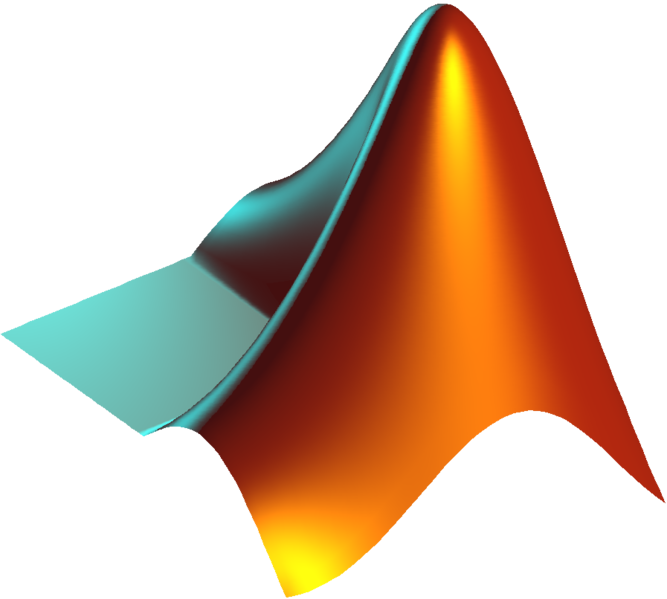
\includegraphics[width=1\textwidth]{images/matlab}
                \end{figure}
            \end{column}
            \begin{column}{0.33\textwidth}
                \begin{figure}
                    \centering
                    
\includegraphics[width=1\textwidth]{images/excel}
                \end{figure}
                \begin{figure}
                    \centering
                    
\includegraphics[width=1\textwidth]{images/idm}
                \end{figure}
            \end{column}
            \begin{column}{0.33\textwidth}
                \begin{figure}
                    \centering
                    
\includegraphics[width=1\textwidth]{images/powerpoint}
                \end{figure}
                \begin{figure}
                    \centering
                    
\includegraphics[width=1\textwidth]{images/photoshop}
                \end{figure}
            \end{column}
        \end{columns}
    \end{frame}

    \begin{frame}{Akin to Stealing}
        \centering
        \begin{LARGE}
            It's a serious CRIME!
        \end{LARGE}
    \end{frame}

    \begin{frame}{Akin to Stealing}
        \centering
        \begin{Huge}
            $\$150,000$
        \end{Huge}
        \vfill{}
        \begin{Huge}
            Jail time of 5 Years
        \end{Huge}
    \end{frame}

    \begin{frame}
        \centering
        \begin{Huge}
            Most of us can't afford them...
        \end{Huge}
    \end{frame}

    \begin{frame}
        \centering
        \begin{Huge}
            But we need to use them, right?
        \end{Huge}
    \end{frame}

    \begin{frame}
        \centering
        \begin{Huge}
            So, what do we do?
        \end{Huge}
    \end{frame}

    \begin{frame}
        \centering
        \begin{Huge}
            Open Source to the rescue!
        \end{Huge}
    \end{frame}

    \begin{frame}{So what's open source}
        \begin{Huge}
            Closed Source
        \end{Huge}

        A resturant that offers delicious food for some money and doesn't give you the recipe

        \vfill{}

        \begin{Huge}
            Open Source
        \end{Huge}

        A resturant that offers delicious food for free and also gives you the recipe
    \end{frame}

    \begin{frame}{A little techincal.. Sorry}
        \lstinputlisting[language=C]{hello.c}
        \begin{figure}
            \centering
            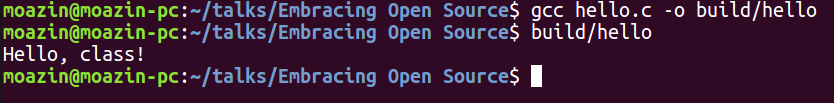
\includegraphics[width=1\textwidth]{images/build}
        \end{figure}
    \end{frame}

    \section{Let's look at some alternatives}
    \begin{frame}{The Office Stack}
        \begin{columns}[T]
            \begin{column}{0.33\textwidth}
                \begin{figure}
                    \centering
                    
\includegraphics[height=0.1\paperheight]{images/word}
                    \caption{MS Word}
                \end{figure}
                \begin{figure}
                    \centering
                    
\includegraphics[height=0.1\paperheight]{images/excel}
                    \caption{MS Excel}
                \end{figure}
                \begin{figure}
                    \centering
                    
\includegraphics[height=0.1\paperheight]{images/powerpoint}
                    \caption{MS Powerpoint}
                \end{figure}
            \end{column}
            \vrule{}
            \begin{column}{0.33\textwidth}
                \begin{figure}
                    \centering
                    
\includegraphics[width=0.25\textwidth]{images/libre-writer}
                    \caption{LibreOffice Writer}
                \end{figure}
                \begin{figure}
                    \centering
                    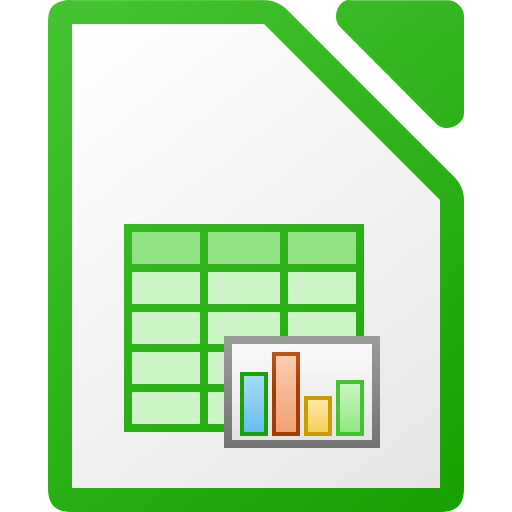
\includegraphics[width=0.25\textwidth]{images/libre-calc}
                    \caption{LibreOffice Calc}
                \end{figure}
                \begin{figure}
                    \centering
                    
\includegraphics[width=0.25\textwidth]{images/libre-impress}
                    \caption{LibreOffice Impress}
                \end{figure}
            \end{column}
            \begin{column}{0.33\textwidth}
                \begin{figure}
                    \centering
                    
\includegraphics[width=0.25\textwidth]{images/google-docs}
                    \caption{Google Docs}
                \end{figure}
                \begin{figure}
                    \centering
                    
\includegraphics[width=0.25\textwidth]{images/google-sheets}
                    \caption{Google Sheets}
                \end{figure}
                \begin{figure}
                    \centering
                    
\includegraphics[width=0.25\textwidth]{images/google-slides}
                    \caption{Google Slides}
                \end{figure}
            \end{column}
        \end{columns}
    \end{frame}


    \begin{frame}{Computations and Simulations}
        \begin{columns}
            \begin{column}{0.5\textwidth}
                \begin{figure}
                    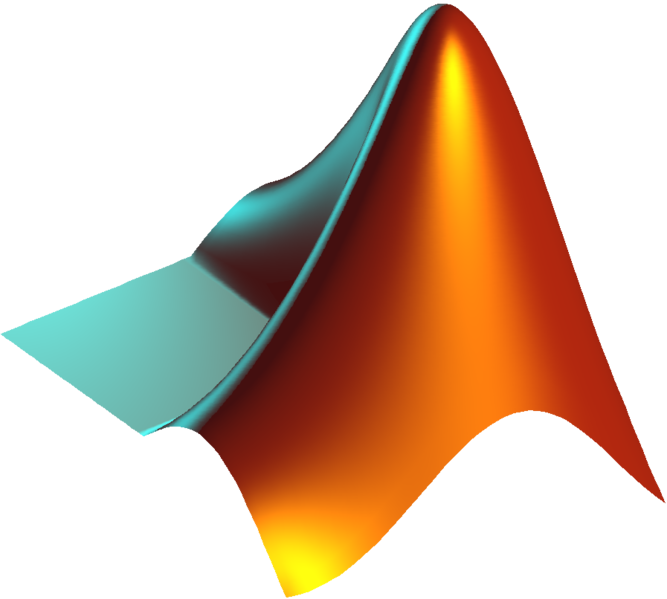
\includegraphics[width=0.5\textwidth]{images/matlab}
                    \caption{MATLAB}
                \end{figure}
            \end{column}
            \vrule{}
            \begin{column}{0.5\textwidth}
                \begin{figure}
                    
\includegraphics[height=0.2\paperheight]{images/octave}
                    \caption{GNU Octave}
                \end{figure}
                \begin{figure}
                    
\includegraphics[height=0.2\paperheight]{images/scilab}
                    \caption{Scilab}
                \end{figure}
            \end{column}
        \end{columns}
    \end{frame}

    \begin{frame}{Creative Suite}
        \begin{columns}
            \begin{column}{0.5\textwidth}
                \begin{figure}
                    
\includegraphics[height=0.12\paperheight]{images/photoshop}
                    \caption{Adobe Photoshop}
                \end{figure}
                \begin{figure}
                    
\includegraphics[height=0.12\paperheight]{images/Illustrator}
                    \caption{Adobe Illustrator}
                \end{figure}
                \begin{figure}
                    
\includegraphics[height=0.12\paperheight]{images/lightroom}
                    \caption{Adobe Lightroom}
                \end{figure}
            \end{column}
            \vrule{}
            \begin{column}{0.5\textwidth}
                \begin{figure}
                    
\includegraphics[height=0.12\paperheight]{images/gimp}
                    \caption{GNU Gimp}
                \end{figure}
                \begin{figure}
                    
\includegraphics[height=0.12\paperheight]{images/inkscape}
                    \caption{Inkscape}
                \end{figure}
                \begin{figure}
                    
\includegraphics[height=0.12\paperheight]{images/rawtherapy}
                    \caption{Raw Therapee}
                \end{figure}
            \end{column}
        \end{columns}
    \end{frame}

    \begin{frame}{Operating Systems}
        \begin{columns}
            \begin{column}{0.5\textwidth}
                \begin{figure}
                    
\includegraphics[height=0.3\paperheight]{images/windows}
                    \caption{Microsoft Windows}
                \end{figure}
            \end{column}
            \vrule{}
            \begin{column}{0.5\textwidth}
                \begin{figure}
                    
\includegraphics[height=0.12\paperheight]{images/ubuntu}
                    \caption{Canonical Ubuntu}
                \end{figure}
                \begin{figure}
                    
\includegraphics[height=0.12\paperheight]{images/mint}
                    \caption{Mint}
                \end{figure}
                \begin{figure}
                    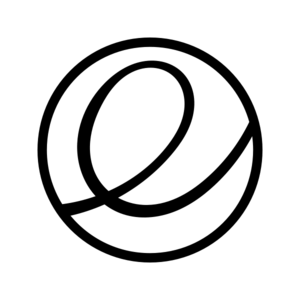
\includegraphics[height=0.12\paperheight]{images/elementaryos}
                    \caption{Elementary OS}
                \end{figure}
            \end{column}
        \end{columns}
    \end{frame}
    
    \begin{frame}
        \begin{Huge}
            We have barely scratched the surface...
        \end{Huge}
    \end{frame}

    \begin{frame}
        \begin{Huge}
            Okay...
        \end{Huge}
    \end{frame}

    \begin{frame}
        \begin{Huge}
            But it's hard right...
        \end{Huge}
        \begin{figure}
            
\includegraphics[width=0.5\textwidth]{images/tired}
        \end{figure}
    \end{frame}

    \begin{frame}
        \begin{figure}
            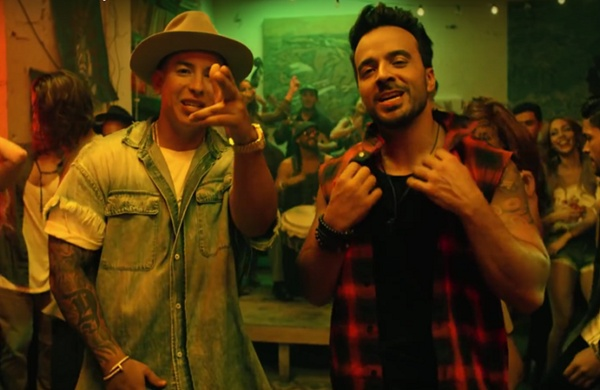
\includegraphics[width=1\textwidth]{images/pacito}
            \caption{Pacito Pacito... Despacito}
        \end{figure}
    \end{frame}

    \begin{frame}
        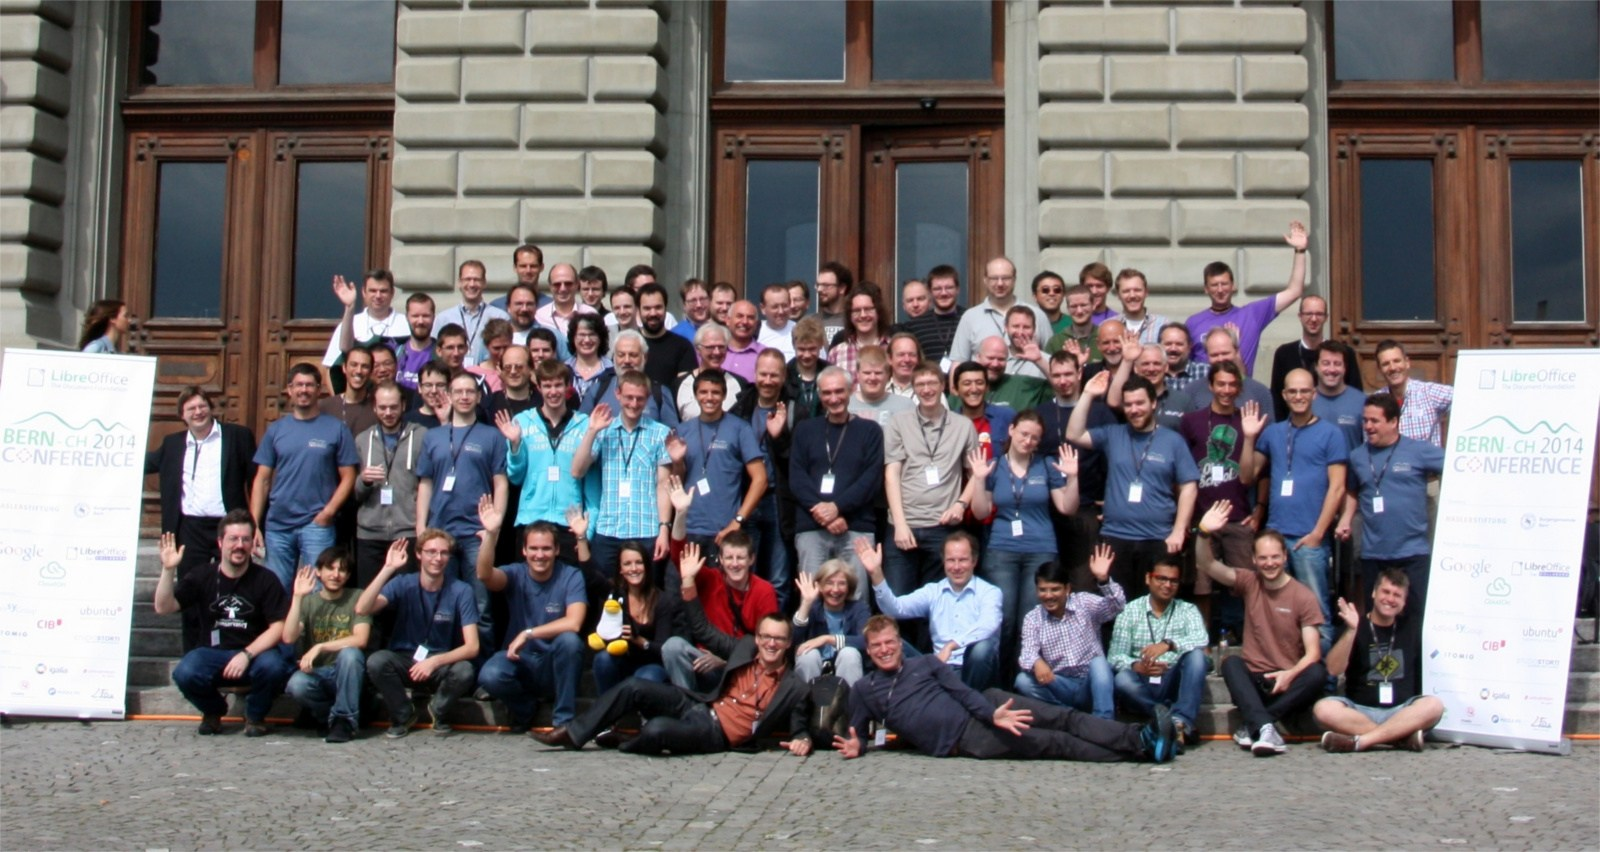
\includegraphics[width=1\textwidth]{images/community1}
    \end{frame}
    \begin{frame}
        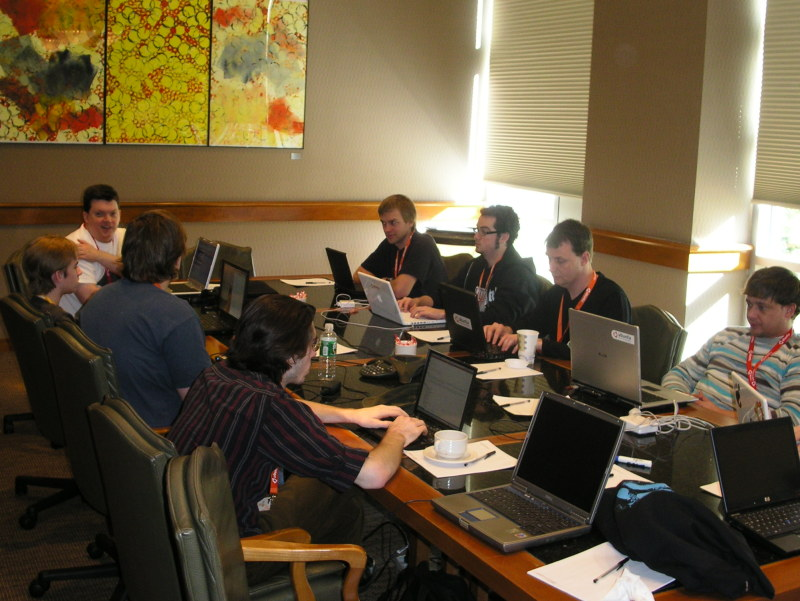
\includegraphics[width=1\textwidth]{images/community2}
    \end{frame}
    \begin{frame}
        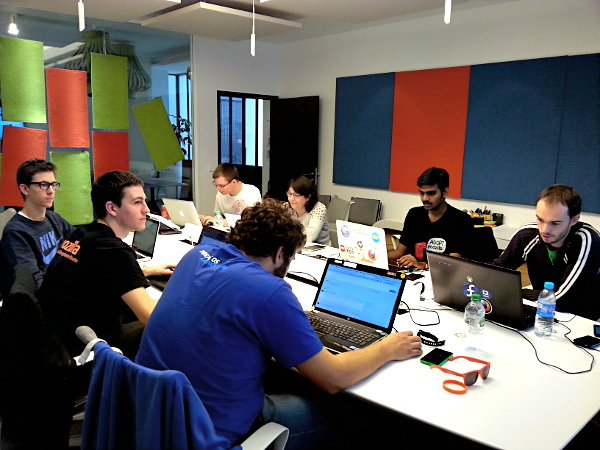
\includegraphics[width=1\textwidth]{images/community3}
    \end{frame}

    \begin{frame}[standout]
        \begin{Huge}
            Questions?
        \end{Huge}
    \end{frame}

\end{document}